\label{sec:risk-assessment}
The following tables identify various risks and hazards associated with the use of our aircraft, following a standard University of Melbourne Risk Assessment template, shown in Figure \ref{fig:risk-matrix}.\\

Each row of the risk assessment tables contains the following information: the potential hazard, the likelihood of that hazard occurring during the mission, a ``rating'' of the consequence of that hazard, and an assessment of the overall risk for that hazard. Management and mitigation of these risks will be discussed in Section \ref{sec:risk-management}.

\begin{figure}[H]
	
	\begin{subfigure}{\linewidth}
		\centerline{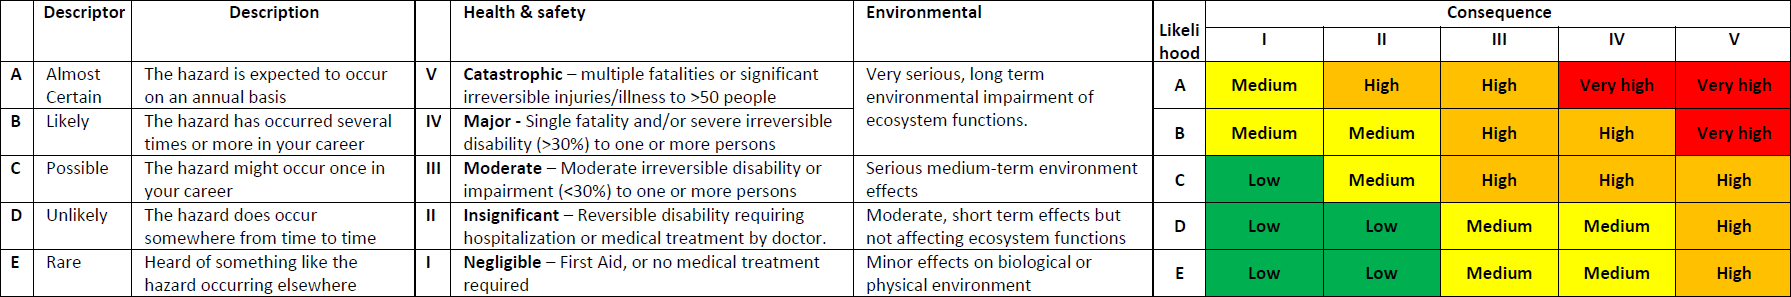
\includegraphics[width=550pt]{../Images/risk-matrix}}
	\end{subfigure}\\[2ex]
	
	\begin{subfigure}{\linewidth}
		\centerline{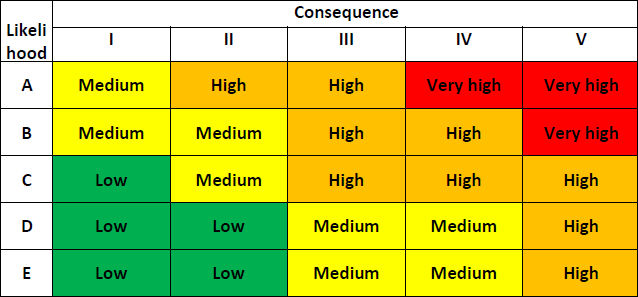
\includegraphics[width=300pt]{../Images/risk-matrix-2}}
	\end{subfigure}
	
	\caption{Risk Management Matrix}
	\label{fig:risk-matrix}
\end{figure}

It would be assumed a UAV would take off shortly after having been turned on and armed. No matter how well pre-arm tests go there is always a chance for failure in flight. As such the UAV could fly erratically immediately after take off and potentially harm nearby people while flying at low altitudes.
This is easy to combat at the home site with line of sight and a kill switch, however during automated landings near Jo we must rely GCS feedback and a kill switch. The one minute buffer between arming and takeoff at Jo’s end will ensure Jo is well clear of the drone further minimising risk.
On landing special care needs to be taken to ensure landing sites are clear of people. Computer vision will to a degree be able to assess suitability of landing sites, but it searches for people based on simple parameters such as clothing colour. We should therefore make the assumption that humanoid figures outside of the mission specs (i.e. anyone that is not Jo) are invisible to the UAV. So due diligence must taken to ensure the UAV is designated to land in the allocated sites and that those sites are well clear during takeoff and landing procedures.
Premature Arming of props while personnel are in close proximity of the UAV is a possible cause of risk as a person must Arm the safety switch on the drone before it can be armed. If the safety switch is pressed by a team member and the UAV is armed in Auto Mission Mode by the Ground Control Station, the arming team member is at risk of injury from spinning props. To ensure safety strong communication between Switch Arming Team Member (SATM) and Ground Control Station Member (GCSM) will be required.

\begin{table}[!h]
	\label{tab:risks-electrical}
	\centering
	\begin{tabularx}{\textwidth}{|Y|c|c|c|}
		\hline
		\textbf{Risk} & \textbf{Likelihood} & \textbf{Consequence} & \textbf{Risk Rating}\\
		\hline
		Electrocution & Possible & Insignificant & Medium\\
		\hline
		Impact to batteries, causing explosion & Possible & Insignificant & Medium\\
		\hline
		Loss of motor power & Possible & Insignificant & Medium\\		
		\hline
	\end{tabularx} 
	\caption{Risk Assessment - Electrical Hazards}
\end{table}

\begin{table}[!h]
	\label{tab:risks-autonomy}
	\centering
	\begin{tabularx}{\textwidth}{|Y|c|c|c|}
		\hline
		\textbf{Risk} & \textbf{Likelihood} & \textbf{Consequence} & \textbf{Risk Rating}\\
		\hline
		& & & \\
		\hline
	\end{tabularx} 
	\caption{Risk Assessment - Autonomous Takeoff and Landing}
\end{table}

\begin{table}[!h]
	\label{tab:risks-inflight}
	\centering
	\begin{tabularx}{\textwidth}{|Y|c|c|c|}
		\hline
		\textbf{Risk} & \textbf{Likelihood} & \textbf{Consequence} & \textbf{Risk Rating}\\
		\hline
		Loss of aircraft control & \MULTROW{Possible} & \MULTROW{Insignificant} & \MULTROW{Medium} \\
		(Autopilot failure or lock-up) & & & \\
		\hline
		Loss of aircraft control  & \MULTROW{Likely} & \MULTROW{Insignificant} & \MULTROW{Medium} \\
		(Propeller or power loss) & & & \\
		\hline
		Loss of GPS link only to GCS & Likely & Insignificant & Medium \\
		\hline
		Loss of telemetry/radio link only to GPS & Likely & Insignificant & Medium \\
		\hline
		Loss of both telemetry and GPS to GCS & Possible & Insignificant & Medium \\
		\hline
		GCS failure & \MULTROW{Possible} & \MULTROW{Insignificant} & \MULTROW{Medium}\\
		(aircraft loses communication with GCS) & & & \\
		\hline
		Geofence breach & Likely & Insignificant & Medium \\
		\hline
	\end{tabularx} 
	\caption{Risk Assessment - In-flight Hazards}
\end{table}

\begin{table}[!h]
	\label{tab:risks-other}
	\centering
	\begin{tabularx}{\textwidth}{|Y|c|c|c|}
		\hline
		\textbf{Risk} & \textbf{Likelihood} & \textbf{Consequence} & \textbf{Risk Rating}\\
		\hline
		Aircraft not operational or not controllable & Possible & Insignificant & Medium \\
		\hline
		Risk of injury to persons near aircraft & Possible & Insignificant & Medium \\
		\hline
	\end{tabularx} 
	\caption{Risk Assessment - General Hazards}
\end{table}